\chapter{Related Work}
Remote sensing \cite{two} with the unmanned aerial systems (UAS) through multispectral imagery dates back to 2008 \cite{eight-icuas} and even earlier where results were generated using traditional approaches of using high cost wide band multi-spectral cameras with application of physical filtering. The field is now emerging with applications which systematically apply monitoring of vegetation and crops to enable well-informed decisions by the farmers in the agricultural activities. The field had a lot of dependence on satellite imagery for collection of hyperspectral data but has observed a paradigm shift to cheaper UAS based solution which are able to gather large amounts of raw data to process for monitoring crop health in more than one way, such as water level concentration identification \cite{two-remotev2}, vigor analysis \cite{three-remotev2}, biomass estimation and disease monitoring using algorithmic analysis based on data from hyperspectral and thermal imagery as well as using machine learning applications of clustering (unsupervised) and supervised learning by collection of large amounts of labelled data of particular fields.  
\\
\\
Both multispectral analysis and the hyperspectral analysis requires acquisition of data aerially at a fixed position in altitude and coverage of the entire crop field using low cost passive imagery sensors such as the normal visible light (RGB) camera, Near Infra Red (NoIR) camera and relatively expensive hyperspectral cameras. The sensors are distinguished by the bands (channels) of electromagnetic spectra captured by them. The spatial distribution of the energy reflected by the plants to these sensors differ in the bands of frequency which points to the variation of plant health spatially in the crop field. The multispectral imagery ranges from wide bands 5 to 12 represented as pixels. The hyperspectral imagery has hundreds or even thousands of bands present as narrow width bands (5-20 nm each). The multispectral imagery we use is a tuned inexpensive version of the expensive multispectral imagery by focusing on the most significant band for chlorophyll level indication, i.e., the Near IR band. The solution can be used by removing the IR filter present in RGB cameras for the camera to capture the Near IR energy spectrum reflected by the crops as well. This can be isolated from the RGB bands by using a band filter for one of the three visible bands. We used a Red light filter for the same. We also have the availibitlity of Red Edge Spectrum using this camera which can yield the NDRE (Normalized Difference Red Edge) results.
\begin{figure}[H]
    \centering
    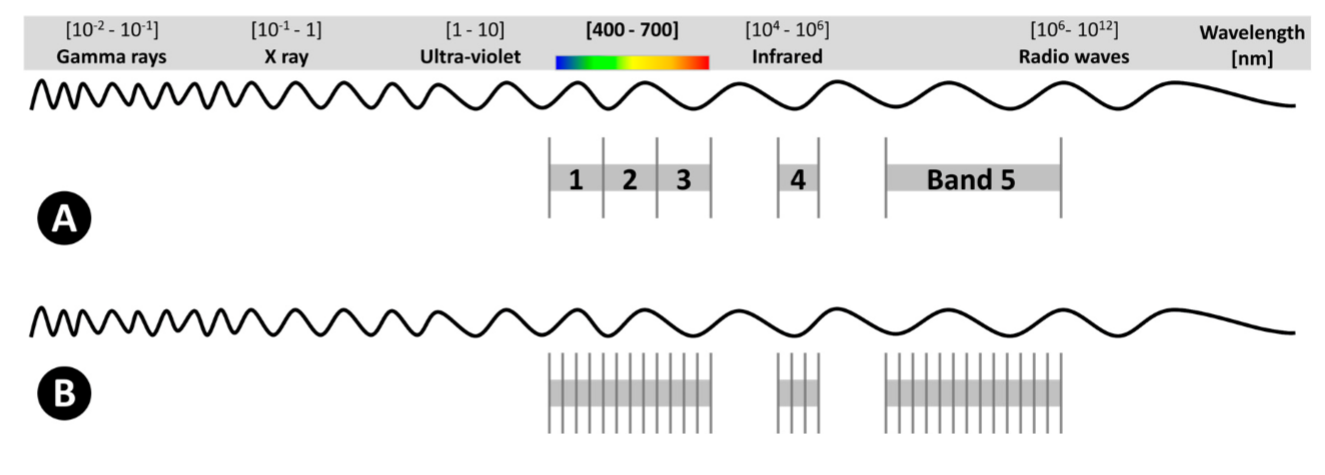
\includegraphics[width=0.7\linewidth]{SummerInterReport/project/Images-Major/em_spectra.png}
    \caption{Spectrum representation including: (A) Multispectral example, with 5 wide bands; and (B) Hyperspectral example consisting of several narrow bands that \cite{fourteen-remotev2}).}
    \label{fig:Concise Flow}
\end{figure}

\\
\\

Multispectral and Hyperspectral imagery can be a boon to the agricultural sector due to their potential to assess even the smallest details such as telling the elemental deficiency in the spatial context of the crop to enable precision farming for the individuals. Also, productivity and stress indicators in agricultural systems can be assessed through photosynthetic light using efficiency quantification, which can be obtained by measuring the Photochemical Reflectance Index (PRI) relying on narrow band absorbance of xanthophyll pigments at 531 and 570nm \cite{fifteen-remotev2}.  However commercial hyperspectral cameras even without the acquisition systems and the data processing systems cost upwards of 6000\$, deeming it unfeasible in Indian conditions where the info-graphic of a higher detail would cost leaps and bounds more to the farmer as well as would be non-usable due to the higher levels of complexity in data, incomprehensible to a large majority (62\% are uneducated as cited by 2012 reports of Times Of India\cite{stats3}). Commercial multispectral systems cost up to 5000\$ or Rs 3.5 lac. However, we successfully managed to reduce the expenditure in our system for data acquisition as well as processing to Rs 3000 or 50\$ (using a raspberry Pi 3B+, supporting expansion in ML domains as well for clustering the hyperspectral imagery in future) and a NoIR camera.
\\
\\
Furthermore, we have used the APM 2.8 flight controllers and tested the algorithms of path planning with Primus V3R in constrained environments as well as CC3D mini, which are all cheaper than the commonly used PixHawk or Pixhack flight controllers.



